% Remove the oneside option below for double sided printing (e.g. for final (post-viva) submission)
\documentclass[a4paper,12pt,oneside,openright]{book}

% Preamble commands go here
\usepackage{customisations}

%% Some of the below packages may be useful to thesis writers in Physics
%% Googling `latex <packagename>' will usually give you some documentation
% \usepackage[load-configurations=abbreviations]{siunitx} % siunitx typesets physical units in a consistent manner
\usepackage{booktabs} % booktabs provides professional formatting commands for tables
\usepackage{amsmath} % amsmath provides extra maths symbols
\usepackage{amsfonts}
\usepackage{textcomp} % textcomp provides extra text symbols (like a degrees celsius symbol)
\usepackage{listings}
% \usepackage{tikz} % tikz is a package for drawing diagrams and adding annotations to figures
% \usepackage{threeparttable} % threeparttable allows for adding notes to tables
% \usepackage{eps2pdf} % eps2pdf allows background transformation of eps files to pdfs so they 
%						work seamlessly with pdflatex. If using this with the LaTeX editor Kile,
%						you need to add --shell-escape before '%source', in
%						Settings -> Configure Kile... -> Tools -> Build -> build_pdflatex

% End preamble

% REPLACE THESE with your thesis title, your name and the date of submission of the thesis
\title{On Interacting Particles in 1D and 2D}
\author{Joshua DM Hellier}
\date{July 2018} % of submission

\newcommand{\partDeriv}[2]{\frac{\partial #1}{\partial #2}}
\begin{document}

% Thesis front matter - title page, abstract, acknowledgements, declaration and table of contents
% See customisations.sty to modify the title page or declaration
\singlespacing
\maketitlepage
\frontmatter
\eighteenptleading
\chapter{Abstract}

Diffusion processes are pretty ubiquitous across the natural world, so it is important to try to understand them. A system in which diffusion is being driven by concentration differences between boundary reservoirs is a simple example of a nonequilibrium statistical mechanics system. In this thesis, we study a model that has been hanging around the literature in one form or another for a long time: the Sticky Particle Model, or SPM. This is a very basic one-parameter exclusion model, in which particles move away from adjacent particles with a different rate to their normal free movement. We use a variety of techniques to analyse induced flow in this model, including a simple analytic mean-field theory, Monte Carlo calculations, and direct numerical analysis of the transition rate operator 
that specifies small versions of the system. During these investigations, we have discovered what we argue is a nonequilibrium phase transition between flow regimes at high and low values of our “stickiness parameter”; much of our work has gone into attempts to understand the nature of this apparent transition.


\singlespacing
% Uncomment this line if you need to declare published work which forms part of the thesis
\declarationpublications{}
\makedeclaration

\chapter{Acknowledgements}

\noindent

\normalsize

I would like to thank Giulio de Magistris, Alexander Slowman, Tom Ives, James Gratrex, Chay Patterson,
Pattanasak Teeratchanan, Yarden Brody, Andreas Hermann, Miguel Martinez-Canales, Eugene Gregoryanz,
Martin Evans,
Richard Blythe, Bartek Waclaw and anyone else I may have missed out for their helpful input during this research project. I am also very
grateful to my parents and friends for their support during what has been a rather difficult time.
Most of all I would like to thank my supervisor, Graeme Ackland, who has contributed a lot of his time
and effort to produce the work you see before you today.



\cleardoublepage
\phantomsection
\addcontentsline{toc}{chapter}{\contentsname}
\setcounter{tocdepth}{2}
\tableofcontents

\cleardoublepage
\phantomsection
\addcontentsline{toc}{chapter}{\listfigurename}
\listoffigures

\cleardoublepage
\phantomsection
\addcontentsline{toc}{chapter}{\listtablename}
\listoftables

% Include main matter here
\mainmatter
\eighteenptleading
\chapter{Preliminary Work, Background and Motivation}

Here we need to talk about the original intent of the project.

\section{The Ti$\text{O}_\mathbf{2}$/Ti Interface System}

A description of the initial problem upon which the project was based.

\section{Initial Attempts to Model the Ti$\text{O}_\mathbf{2}$/Ti Interface System}
\subsection{The Difficulties of Nonequilibrium Statistical Mechanics}
\subsection{Dynamics of Ionic Crystals}
Maybe mention Ewald sums, and the other issues with computations about materials.
\subsection{Initial Work Done with MD}
I used some LAMMPS code to try to work with MD initially; melts and things.
\subsection{The Problems with MD}
Need to explain why issues with using MD, and why I eventually decided it was not a useful technique for this problem; in particular, why MD is fundamentally flawed as a concept.

\section{Simple Large-Scale Models of the Ti/O/Nb Interacting System}
I had a think about various methods I could use to tackle the system in question, and decided that the approach would would be most likely to bear fruit would be a continuum-modelled bulk PDE system with appropriate boundary conditions between
phases.
\subsection{Proposed Linear System}
Simplest possible model, and why it failed.
\subsection{Attempts to create a Suitable Nonlinear System}
Talk about why nonlinearity is necessary (as in, it just spits out the previous system again), and the difficulties of parametrising it.
\subsection{Parametrisation from a Microscopic Model}
Talk about the Dresden conference and what I learned from it.

\section{The Sticky Particle Model}
\subsection{Model Motivation}
As in, why this is a good start in 1d.
\subsection{Model Definition}
\subsection{Model Properties}
Including Detailed Balance, symmetry, ``locality''. Also mention that it is a Markov process.
\subsection{Relation to Existing Literature}
\subsection{Generalisation to Higher Dimensions}
Including a proof of detailed balance in arbitrary dimensions (on square lattice).

\section{Implications of Initial Work for the PhD Direction}
\subsection{Why the Change of Direction?}
Essentially, why trying to solve this particular problem is actually kind of silly, and why having a better theory of driven lattice flows would be more useful.
\subsection{Why Investigate Flow in the SPM?}
Talk about how boundary-condition-induced flow on systems that would otherwise obey detailed balance hasn't really been done before.
Bring it around to the question:
``Can we have interesting dynamics in a model which is symmetric and obeys detailed balance?''
\chapter{Analytical Results about the SPM} \label{sec:analChap}

We now have a model, the SPM, which should represent the kind of behaviour in which we are interested.
In this chapter, we will attempt to derive analytic results about how particles flow in the model. Initially,
this was all done with the aim of
producing an approximation to the behaviour in the hydrodynamic limit and thus informing us about phenomena such as surface layer formation; however, as you will see the analytic
predictions suggest that the flows could be quite interesting in their own
right.

\section{Solving Problems in Nonequlibrium Statistical Mechanics}
Models in nonequlibrium statistical mechanics which contain nontrivial interactions between components often produce interesting behaviour, hence the wide interest in these models. However, they usually prove to be difficult to ``solve'' in any
concrete sense. In this section, I will give a brief overview of solution methods in equilibrium statistical mechanics, why nonequilibrium statistical mechanics problems tend to be harder to solve, and how this affects the way we approach
the SPM.


\subsection{Equilibrium Statistical Mechanics}
Equilibrium statistical mechanics is a bread-and-butter part of undergraduate physics, and there are a great many texts on the subject~\cite{landauLifshitzStatmech, reif2009}.
When we speak of ``solving'' an equilibrium statistical mechanics system, the gold standard is to be able to calculate relationships between the statistics of large-scale quantities as a function of the system constraints or their conjugates.
This allows one to classify the system's behaviour by making equations of state  and identifying phase transitions, situations where at least some large-scale quantity statistics vary with respect to each other in a discontinuous manner.
As you will see, the SPM itself is isomorphic to an equilibrium statistical mechanics model so long as we do not drive the system using boundary conditions (e.g. particle reservoirs with different concentrations). Once we introduce such driving forces, however, we find that we can no longer use
equilibrium analysis, and things get a bit more difficult.
% would like to write about the ideal gas and Ising model here
\subsubsection{Exact Solutions}
A quantity of key interest in equilibrium statistical mechanics is the partition
function~\cite{martynovStatmech}, usually denoted by $Z$. Say we have a closed classical mechanical system maintained at constant temperature $T$ by a heat bath,
so only energy can enter and leave the system (the canonical ensemble). Let its state space be $\Xi$, and denote an individual microstate (specific configuration of the system) by $\xi$.
Such a system is defined by a Hamiltonian $H : \Xi \rightarrow \mathbb{R}$. The canonical partition function for this system is defined to be
\begin{equation} \label{eq:partFn}
 Z(\beta) = \int_\Xi  \! \! \mathrm{d}  \xi \  \  e^{- \beta H(\xi)},
\end{equation}
with $\beta T = 1$, where the integrand on the right hand side is the familiar Boltzmann weighting. This quantity is extremely useful, because it and its derivatives are directly related to the statistics of large-scale quantities.
For example, the ensemble-averaged total energy $\langle E \rangle$ satisfies
\begin{equation}
 \langle E \rangle = - \partDeriv{\log{Z}}{\beta}
\end{equation}
If one is able to obtain an expression for the canonical partition function by analytic means, you can calculate essentially any statistical moment of any large-scale quantity (\textbf{state variable})
you desire, and thus the system is ``solved'' in the sense used above.



\subsubsection{Approximate Methods for Analysing Equilibrium Statistical Mechanics Systems}
Of course, the situation in which one can simply evaluate the partition function exactly is
extremely rare in equilibrium statistical mechanics, at least in the large-scale limit (the one of
principal interest, as it is required for most interesting phenomena such as phase transitions).
More often, one might approximate the partition function itself, perhaps by converting the required
integral (Eq. \eqref{eq:partFn}) into an asymptotic series in one of the thermodynamic variables;
this is essentially what one does when analysing a system in terms of instanton transitions~\cite{grafke2015}.

Another approach is to deal directly with the state variables we are interested in themselves,
and try to find approximate relationships between them in order to classify their interdependence (an
\textbf{equation of state}). Equilibrium mean-field theory
(\textbf{MFT})~\cite{honig1999} is exactly such a method.
In MFT, we introduce the means of thermodynamic quantities of interest as independent
variables, and then make the assumption that they have no nontrivial correlations. In practical terms,
this means that for thermodynamic variables $x$ and $y$, we assume that
\begin{equation}
 \left\langle x y \right\rangle = \left\langle x  \right\rangle \left\langle y \right\rangle.
\end{equation}
This is of course quite an assumption to make, although it is often the case that it is true to low
order in some asymptotic expansion. Typically, MFT tends to work well in higher dimensions and more
weakly correlated systems. In the case of the Ising Model (the Weiss Molecular Field~\cite{van1945}), it incorrectly predicts a phase transition
in $1$D, but for $2$D and above it is at least qualitatively correct.

Finally, one can attempt to sample directly from the space of microstates numerically via Monte Carlo
methods, and in doing so build up information about state variables that way.
We will say more about this in Ch. \ref{sec:numerics}.

\subsection{Nonequlibrium Statistical Mechanics}
Nonequilibrium statistical mechanics differs from equilibrium statistical mechanics in the sense that
it is ``out of equilibrium''. The actual meaning of this is that there are nontrivial currents
(be they of energy, matter, or otherwise) flowing through the system. Note that it is perfectly
possible for a nonequilibrium statistical mechanical system to be out of equilibrium but still in a
steady state, in the sense that the system's microstate can be constantly changing but still
maintaining a fixed time-averaged ensemble distribution, allowing currents to flow.

In general, nonequilibrium statistical mechanics problems tend to be quite a lot harder to get 
a handle on than equilibrium statistical mechanics problems. The principal reason for this is the
issue of time-dependence. In true equilibrium, where there is no flow and therefore no overall motion,
there is no passage of time, which effectively reduces the number of variables under consideration. This, coupled with the second law of thermodynamics, means that whatever state we are
in must be an allowed state with maximal entropy; in this case, entropy ends up acting a little bit
like a Lyapunov function~\cite{pukdeboon2011}, which we can use to find candidate final states. 

This is of no help to us at all out of equilibrium: asking a question such as
``how much current flows across a given concentration gradient?'' inherently involves time, and so
we can't just make a maximal-entropy argument to get the answer. There are occasions in the 
literature where a principle of ``maximal entropy production''~\cite{dewar2005, martyushev2006}
is invoked in order to close sets of
equations, but as far as we have seen there is not yet a proof of why such a thing should in
general be true.


\subsubsection{Exact Solutions}
Some problems in nonequilibrium statistical mechanics are known which have exact solutions. 
These include the Ising model in $1$ and $2$ dimensions~\cite{brush1967}, as well as a class of problems which can be
solved in steady state by matrix products or Bethe ansatz~\cite{van2016}. 
These are the subject of much
interest at the
moment, not least because one can often use isomorphisms between systems which are known to
be integrable in order to discover new integrable systems~\cite{Rota1989}.
Unfortunately, building up such an exact solution to a specific problem from scratch does not seem to be possible in every case,
so it remains to be seen how useful these methods really are for tackling problems of actual
physical interest.


\subsubsection{Approximations}
As with equilibrium statistical mechanics, there are a bunch of approximate methods which can
be invoked to probe system behaviour, some of which we have used in our research.
Instead of solving the full system as an integrable system, there are approaches in which instantons
are used to ``patch together'' local solutions to try to get a grasp of the whole picture
~\cite{wallace1978}. One can,
as always, simply simulate a system by numerical means and try to derive useful statistics from the
output. In order to do this more efficiently, one can possibly use results from Large Deviation
Theory (LDT~\cite{touchette2011}) in order to boost the strength of the tails of the distributions and so capture the essence
of some useful large deviation function. However, again this doesn't seem to be something that can
be done completely generically.

Of course, mean-field theory is still an option, although now that time dependence has been added
it tends to produce a set of coupled ODEs for the mean variables under consideration~\cite{Kolesnichenko2014}. It is also in
principle possible to study small-scale systems essentially exactly by numerical analysis of the
relevant \textbf{Transition Rate Matrix} (TRM). Of course, this has the disadvantage that it is only a
small finite system, so some of the phenomena observed in it will differ from larger versions of the
same system. We perform this kind of analysis in Ch. \ref{sec:transRateChapter}.


\subsection{Where does the SPM stand?} \label{sec:spmStatus}
The issue of how to analyse the SPM leaves us in a slightly awkward position. It is almost as simple
as the Symmetric Exclusion Process; however, the extra interaction in the SPM makes it quite
different, as it is in fact longer-ranged. Thus, it is a bit difficult to see immediately how to
modify a SEP matrix-product steady state in order to solve the SPM. In a similar vein, it might 
in fact be possible to solve the SPM exactly using the thermodynamic Bethe ansatz~\cite{van2016},
but we have neither
the expertise nor the time to properly investigate that possibility.

Instead, we have gone for a somewhat more pedestrian, traditional approach. In the rest of this
chapter, we will discuss the relationships enjoyed by the SPM and some well-known models,
and will then perform  mean-field analysis, in the hope of obtaining some at least qualitative
results about how the SPM behaves. In Ch. \ref{sec:transRateChapter}, we will then consider some semianalytic solutions to the SPM
in finite systems in $1$D via TRM analysis. Finally, in Ch. \ref{sec:numerics}, we will compare the TRM and MFT results to numerical simulations performed using Monte-Carlo (MC) methods. We have also performed
MC calculations and have MFT results for the $2$-dimensional situation.


\section{Similarities between the SPM and Established Models in 1D}
In the previous section we have discussed the various approaches one might use when attempting to derive properties of a nonequilibrium statistical mechanical system. We will now try to put these ideas into practice on the SPM. We already mentioned some of the relationships between the SPM
and some established models in Sec. \ref{sec:existingModels}; here we will be a little more formal
in terms of our use of these models.



\subsection{Relationship with the Ising Model} \label{sec:isingSim}
If we implement the rules of the SPM on a periodic domain, we no longer have to deal with boundary conditions. In this special circumstance, we can find an isomorphism between this model and the Ising model with fixed magnetisation.
One does this by associating the Ising spins $\sigma_i \in \left\{-1, 1 \right\}$ with $\rho_i \in \left\{ 0, 1 \right\}$ via
\begin{equation}
 \rho_i = \frac{1}{2}\left(1+\sigma_i\right).
\end{equation}
Recalling our proof that the SPM obeys detailed balance, we saw that the equilibrium probability of finding the SPM in a state containing $N$ particle-particle adjacencies is proportional to 
$\lambda^{-N}$.
%obviously refer to this
If our Ising Hamiltonian is defined via
\begin{equation}
 H = \frac{1}{2} \sum_{i=1}^L J \sigma_i \sigma_{i+1 \pmod L},
\end{equation}
the probability of finding ourselves in a state with $N$ paired spins is $e^{-\beta N J}$, with $\beta T =1$. The comparison with the SPM is now obvious: we set $\log{\lambda} = \beta J$. Thus $\lambda$ in the SPM has a one-to-one mapping to the ratio of the binding energy to the temperature in the Ising model.


\subsection{Correlation Functions}
For relatively small systems, given a system size $L$ and a number of particles $N$, we can analytically compute the pairwise correlation function $C(l) = \left\langle \rho_i \rho_{i+l} \right\rangle$, or ``the probability that site $i+l$
is occupied given that $i$ is'' (the system is clearly homogeneous in $i$, so its value is irrelevant).
A Python code which performs this calculations is discussed in Sec. \ref{sec:corrFnCode}.


This is quite a nice result, as we can use simple recursion to perform a calculation which would otherwise be quite difficult to code.
Unfortunately the time complexity of the calculation grows exponentially in and $L$, so the largest 
$L$ I can reasonably run for is $20$. In the table below I have plotted the occupation probability of sites shifted from the origin
(normalised so that the correlation with no shift is $1$)  for a selection of $\lambda$ and particle densities.

\begin{figure}[h!]
\caption[Plots of the equal-time particle density correlation function on a ring.]{\label{fig:corrFns}Some particle-particle correlation functions for the SPM on a small closed ring,
with the density fixed by the choice of how many particles to insert at the start. The system in this case has $20$ lattice sites.
This was calculated using computer-assisted algebra and the various density and stickiness combinations should give an overall impression as to their structure.}
\begin{center}
 \begin{tabular}{c  c | c | c | c}
  & $\rho$ & $\frac{3}{20}$ & $\frac{1}{2}$ & $\frac{17}{20}$ \\
  $\lambda$ & & & & \\
 \hline
    \raisebox{3 em}{ $\frac{1}{10}$ } & & \includegraphics[width=0.25\linewidth]{analytics/images/exactCorrFns/lowDensLowL}  & \includegraphics[width=0.25 \linewidth]{analytics/images/exactCorrFns/midDensLowL} & \includegraphics[width=0.25 \linewidth]{analytics/images/exactCorrFns/highDensLowL} \\
    \hline
    \raisebox{3 em}{ $1$ } & &    \includegraphics[width=0.25\linewidth]{analytics/images/exactCorrFns/lowDensMidL}  & \includegraphics[width=0.25 \linewidth]{analytics/images/exactCorrFns/midDensMidL} & \includegraphics[width=0.25 \linewidth]{analytics/images/exactCorrFns/highDensMidL} \\
    \hline
    \raisebox{3 em}{ $10$ } & &    \includegraphics[width=0.25\linewidth]{analytics/images/exactCorrFns/lowDensHighL}  & \includegraphics[width=0.25 \linewidth]{analytics/images/exactCorrFns/midDensHighL} & \includegraphics[width=0.25 \linewidth]{analytics/images/exactCorrFns/highDensHighL} \\
    \end{tabular}
\end{center}
    \vspace{-2em}
\end{figure}

Clearly, as $l$ becomes large, the correlation function tends to the density (note that the way we have defined the correlation function does not subtract this background probability; hence why many definitions do). Very small $\lambda$-values
cause particles to tend to cluster together, whilst large $\lambda$ values cause particles and vacancies to tend to alternate. In theory we could use the equivalence with the Ising model to compute correlation lengths as a function
of $\rho$ and $\lambda$ by using the magnetic field in the original Ising model as a Lagrange multiplier in order to fix the total magnetisation (corresponding to particle number in the SPM). However, due to the fact that we cannot
accurately compute correlation functions to any decent accuracy using our numerics (see Ch. \ref{sec:numerics}), we concluded that it was not worth the time to perform the calculation as we would have nothing to compare it to.


\subsection{Calculation of the Partition Function of the SPM on a Closed Ring} \label{sec:spmPartFn}

Using the duality between the SPM in a closed system and the Ising Model, we
can observe that the probability weighting of any configuration is proportional to $\lambda^{-k}$,
where $k$ is the number of particle-particle adjacencies in the SPM. This raises the question: if we know the weightings, can we calculate the
partition function, and therefore other quantities such as the free energy or chemical potential,
for the SPM on a closed ring with particle density $\rho$?

In order to attempt this, we must first make two observations from the field of combinatorics:
\begin{itemize}
 \item The number of possible ways to select, without ordering or replacement, $M$ objects from $N$
 is
 \begin{equation}
  \begin{pmatrix}
   N \\
   M \\
  \end{pmatrix}
  = \frac{N!}{M!(N-M)!}.
 \end{equation}
\item The number of ways to insert $M$ unlabelled balls into $N$ boxes is
\begin{equation}
 \begin{pmatrix}
  N+M-1 \\
  M-1 \\
 \end{pmatrix}
 = \frac{(N+M-1)!}{N!(M-1)!}.
\end{equation}
 \end{itemize}
Now let us consider an alternative way to look at our SPM system. Instead of considering particles and vacancies
moving
around on a lattice of size $L$, let us instead consider a ring containing $N$ boxes, into which we wish to
distribute $L-N$ balls. These balls are allowed to jointly occupy boxes; this corresponds to the SPM on
a ring with $L$ slots containing $N$ particles. The occupation numbers of the boxes represent the distances 
between consecutive particles in the old system.

Say we wish to distribute the balls so that only $M$ of the boxes
contain any at all; then the above two combinatorial results suggest that there are
$\frac{N!}{M!(N-M)!}$ ways to choose which $M$ boxes, into which we insert one ball each,
leaving $\frac{(L-N-1)!}{(L-N)!(M-1)!}$ ways to insert the remainder. Thus, the overall number of
possible ways to distribute the balls so that only $M$ boxes contain any at all is
\begin{equation}
 C_M = \frac{N!(L-N-1)!}{M!(N-M)!(L-N)!(M-1)!}.
\end{equation}
This corresponds to the situation when there are $(N-M)$ particle-particle adjacencies in the SPM. By analogy with
the Ising model, 
the equilibrium weighting of a configuration in which only $M$ of the boxes are nonempty is
$\lambda^{-(N-M)}$; therefore, the partition function $Z_L (\lambda, N)$ for an SPM system of size $L$ is
\begin{equation}
 Z_L (\lambda, N) = \sum_{M=1}^{M=\min{ \{ N-1, L-N \} }} \left[ \frac{N!(L-N-1)!}{M!(N-M)!(L-N)!(M-1)!}
 \lambda^{-(N-M)} \right].
\end{equation}
For statistical mechanics, we are primarily interested in the situation where the system size is very
large. Therefore, let us define $\rho$, $m \in (0, 1)$ so that $N = \rho L$ and $M = mL$, and invoke
the Stirling approximation $\log{x!} \sim x \log{x}$ for large $x$. Regarding $L$ as a large 
constant, and keeping only leading order behaviour in $L$, we find that 
\begin{equation}
\begin{split}
 Z_L (\lambda, \rho) &\sim \int_{0}^{\min{\{ \rho, 1-\rho \}}} \! \mathrm{d}m \
 \exp{L \left[-2m \log{m} + (1-\rho)\log{(1-\rho)} + \rho \log{\rho} \right.} \\
 & \left. -(1-\rho-m)\log{(1-\rho-m)}
 -(\rho-m)\log{(\rho-m)} - (\rho-m)\log \lambda \right]
 \end{split}.
\end{equation}
This integral looks quite intractable, but recall that in the limit $L \rightarrow \infty$ we can
evaluate it asymptotically using Laplace's Method. This requires finding the location of
extrema of the exponentiated term as a function of $m$; these occur when
\begin{equation}
 \lambda(1-m-\rho)(\rho-m) = m^2 .
\end{equation}
One of the solutions occurs in $(0, \min{\{\rho, 1-\rho\}})$, at 
\begin{equation}
 m_+ = \frac{-\lambda+\sqrt{\lambda^2 + 4\lambda(1-\lambda)\rho(1-\rho)}}{2(1-\lambda)},
\end{equation}
and a little analysis reveals that
it is indeed a maximum, as required for the use of Laplace's Method. Therefore, we find that
\begin{equation}
\sqrt[L]{Z_L (\lambda, \rho)} \sim \sqrt{2 \pi } \frac{  (1-\rho )^{1-\rho } \rho ^{\rho }}{
m_+^{2 m_+} \left(\rho -m_+\right)^{\rho-m_+} \left(1-m_+-\rho
   \right)^{1 - m_+ - \rho}} \left( 1 + \mathcal{O}(L^{-1})  \right) ,
\end{equation}
where the term relating to the curvature of the integrand around the critical point (which would usually be
present when using the Laplace Method) vanishes under the action of the $L^\mathrm{th}$ root for large $L$.
From here one can use computer algebra to obtain the free energy density
$
 F(\rho, \lambda) = - \frac{\log{Z_L}}{L}
$
(Fig. \ref{fig:spmFreeEnergy}) and chemical potential $\mu (\rho, \lambda) = \partDeriv{F}{\rho}$
(Fig. \ref{fig:spmChemPot}) of the SPM system. 
\begin{figure}[h!]
 \caption[The free energy density of the SPM on a closed ring, as a function of density
 and $\lambda$.]{\label{fig:spmFreeEnergy} 
 The variation of the SPM free energy density on a large closed ring as a function of particle 
 density and stickiness parameter $\lambda$. The patches on the line $\lambda=1$ are
 due to the way that $m_+$ is calculated; although a little analysis reveals that it is in fact a
 well-behaved removable singularity, numerical errors cause the plotting numerics to behave
 badly in places.
 }
  \begin{center}
 \includegraphics[width=1.0\textwidth]{analytics/images/spmFreeEnergy}
  \end{center}
\end{figure}

\begin{figure}[h!]
 \caption[The chemical potential of the SPM on a closed ring, as a function of density
 and $\lambda$.]{\label{fig:spmChemPot} 
 The variation of the SPM chemical potential on a large closed ring as a function of particle 
 density and stickiness parameter $\lambda$. Again, we see some bad behaviour at $\lambda=1$,
 for the same reasons as before. The curve $\mu (\rho, \lambda) = 0$ is highlighted by a thick black contour.
 }
  \begin{center}
 \includegraphics[width=1.0\textwidth]{analytics/images/spmChemPot}
  \end{center}
\end{figure}
Of course, in thermodynamic equilibrium a system generally attempts to lower its total free energy
to the lowest value allowed by the constraints. If we hold $\lambda$ constant whilst allowing $\rho$
to vary, this corresponds to the curve $\mu(\rho, \lambda)=0$, which one can follow on
Fig. \ref{fig:spmChemPot}; Fig. \ref{fig:spmFreeEnergy} confirms that this is indeed
a minimum. Thus we should expect that a very large system connected to a particle reservoir would
tend towards having a total density such that $\mu = 0$, regardless of the particle density
in the reservoir, as the particle density in the system would only be pinned to that of the
reservoir near to the boundary. By this logic, at large $\lambda$ we would see systems tend towards a
density of $\rho\sim\frac{1}{3}$, whereas for small $\lambda$ the system would tend to fill.
Of course, if we were to hook a system up to two different boundaries and cause a current to flow,
as we have done many times in the course of this project,
that might change things, as now the system would be in a nonequilibrium steady state as opposed
to a thermodynamic equilibrium, and those are not quite the same beast.

\section{Using the Mean-Field Approximation on the SPM} \label{sec:spmMft}
For the reasons discussed in Sec. \ref{sec:spmStatus}, we do not possess an analytic solution for the SPM on a nonperiodic bounded domain. Such a solution might exist, but
we will proceed on the assumption that the model is not analytically solvable. Therefore, it would be useful to at least possess approximate analytic solutions, as this can help us by giving us
something to test our numerics against, and point us in the direction of interesting behaviours which might occur. We will start by deriving the MFT on a lattice, and will then take the continuum limit (as the lattice spacing tends to zero
relative to our scale of interest), as that should predict the dominant behaviour on the macroscopic scale.


\subsection{Lattice MFT Derivation} 
\label{sec:latticeMFT}
As usual, in an MFT approximation, we will say that the equal-time probability of the $(i+1)^\mathrm{th}$ site being occupied is independent of the probability that the $i\mathrm{th}$ site is occupied.
More formally, let us denote the mean occupation of the $i^\mathrm{th}$ site at time $t$ by $\rho_i (t)$. When we invoke the mean-field approximation, we say that the mean occupations of sites at equal times are independent; thus,
the probability that site $j \ne i$ is occupied given that site $i$ is occupied is $\rho_j (t)$. We can use this to calculate the rate at which $\rho_i (t)$ increases and decreases, and so obtain a system of coupled ODEs for $\rho_i (t)$.

Let us first consider the situation where the $i^\mathrm{th}$ site is unoccupied. The probability of this being the case is $(1-\rho_i (t))$. A particle could move from site $(i-1)$ or site $(i+1)$, but only if those sites are currently occupied.
Assuming that site $(i-1)$ is occupied (occurring with probability $\rho_{i-1}$ in MFT), the rate at which it would jump to site $i$ would depend on the occupation of site $(i-2)$,
as it would be $1$ if it were unoccupied and $\lambda$ if it was occupied. Phrasing this in MFT terms,
and suppressing $t$-dependence for brevity, the rate at which $\rho_i (t)$ is increased by particles coming from the left is
\begin{equation}
{\tau_0}^{-1} \left(1-\rho_i \right) \rho_{i-1} \left[ \left(1-\rho_{i-2} \right) \cdot 1  +   \rho_{i-2} \cdot \lambda \right].
\end{equation}
By symmetry, the income of particles from the right is
\begin{equation}
{\tau_0}^{-1} \left(1-\rho_i \right) \rho_{i+1} \left[ \left(1-\rho_{i+2} \right) \cdot 1  +   \rho_{i+2} \cdot \lambda \right].
\end{equation}
Using similar logic, but shifting things around slightly, the rate at which particles leave site $i$ to go to site $i+1$ is
\begin{equation}
{\tau_0}^{-1} \left(1-\rho_{i+1} \right) \rho_{i} \left[ \left(1-\rho_{i-1} \right) \cdot 1  +   \rho_{i-1} \cdot \lambda \right],
\end{equation}
and similarly 
\begin{equation}
{\tau_0}^{-1} \left(1-\rho_{i-1} \right) \rho_{i} \left[ \left(1-\rho_{i+1} \right) \cdot 1  +   \rho_{i+1} \cdot \lambda \right]
\end{equation}
is the rate at which particles leave $i$ to go to $i-1$.

At this point we introduce the quantity $\zeta = 1-\lambda$, for neatness.
The total rate at which particles enter site $i$ is
\begin{equation}
 {\tau_0}^{-1} \left(1-\rho_i \right) \left[ \left(1-\zeta \rho_{i-2} \right) \rho_{i-1} + \left(1-\zeta \rho_{i+2} \right) \rho_{i+1} \right]
\end{equation}
whilst they leave at rate
\begin{equation}
 {\tau_0}^{-1} \rho_i \left[ \left(1-\zeta \rho_{i+1} \right) \left(1 - \rho_{i-1} \right) + \left(1-\zeta \rho_{i-1} \right) \left(1 - \rho_{i+1} \right) \right]
\end{equation}
Combining the rates of arriving and leaving, we obtain our main result:
\begin{align}
\label{eq:latticeMFT}
\begin{split}
 \tau_0 \partDeriv{\rho_i}{t} &= \left( 1-\rho_i \right) \left[ \left(1-\zeta\rho_{i-2} \right) \rho_{i-1} + \left(1-\zeta\rho_{i+2} \right) \rho_{i+1} \right] \\
 &- \rho_i \left[ 2 \zeta \rho_{i-1} \rho_{i+1}  - (3-\zeta)\left(\rho_{i-1} + \rho_{i+1}\right) + 2 \right].
 \end{split}
 \end{align}
This is a nice result, and in theory we could stop right here and we could make a computational scheme for solving this as a sequence. However, there are a few issues. For one thing, $\rho_i (t)$ isn't the mean of a quantity
whose variance is being suppressed by the law of large numbers, as is desired when using the MFT approximation.
Thus, it is merely a rough sketch of what might happen, as variances and correlations between sites aren't suppressed. On the other hand, it simply relates the occupations of nearby sites,
whereas we would find a description of the bulk flow to be much more useful. Therefore, we may as well take the continuum limit to see how flow depends on concentration gradient and local density.

\subsection{Continuum Limit MFT Derivation}
To take the continuum limit, let's promote $\rho_i (t)$ to $\rho(x, t)$ so that 
\begin{equation}
\rho_{i+m}(t)~\rightarrow~\rho(x+am,t).
\end{equation}
Now we can Taylor expand for $\rho_{i+m} (t)$, as
\begin{equation}
 \rho(x+am,t) = \rho(x, t) + ma \partDeriv{\rho(x, t)}{x} + \frac{1}{2} m^2 a^2 \partDeriv{^2\rho(x, t)}{x^2} + \mathcal{O}(a^3). 
\end{equation}
Preferably with the aid of a computational algebra package (such as Wolfram Mathematica), one may directly substitute Taylor expansions for the required $\rho_j$ into Eq. \eqref{eq:latticeMFT}, continuing to truncate
at $\mathcal{O}(a^3)$. Doing so, and collecting terms, we find that
\begin{align}
  \tau_0 \partDeriv{\rho}{t} =& a^2 \left[ 1-\zeta \rho (4-3\rho) \partDeriv{^2 \rho}{x^2}  \right] +
  2 a^2 \zeta (3\rho-2) \left(\partDeriv{\rho}{x}\right)^2 + \mathcal{O}(a^4) ,
\end{align}
which may be factorised into the more convenient form
\begin{equation}
\label{eq:contPDE}
 \partDeriv{\rho}{t} = \frac{a^2}{\tau_0} \partDeriv{}{x} \left\{ \left[1 - \zeta \rho\left(4-3\rho\right) \right] \partDeriv{\rho}{x} \right\},
\end{equation}
which is a continuity equation
\begin{equation}
 \partDeriv{\rho}{t} = \partDeriv{J}{x} 
\end{equation}
with current
\begin{equation}
J = -\frac{a^2}{\tau_0} \left[1 - \zeta \rho\left(4-3\rho\right) \right] \partDeriv{\rho}{x}.
\end{equation}

Considering Fick's Law
\begin{equation}
 J = - D \partDeriv{\rho}{x},
\end{equation}
we see that our diffusion coefficient is
\begin{equation}
 D = \frac{a^2}{\tau_0} \left[1 - \zeta \rho\left(4-3\rho\right) \right].
\end{equation}
Setting $\zeta \rightarrow 0$ (i.e. $\lambda = 1$), we see that $D \rightarrow \frac{a^2}{\tau_0}$, which is consistent with what we would expect for SEP.

Clearly, the diffusion coefficient varies quadratically with $\rho$. This is easiest to see via a few graphs, as shown in Fig. \ref{fig:analDiffCoeffs}. Note that $D \rightarrow \frac{a^2}{\tau_0}$ as $\rho \rightarrow 0$
and $D \rightarrow \frac{a^2}{\tau_0} \lambda$ as $\rho \rightarrow 1$, so for $\zeta < 0$ ($\lambda>1$) $D$ is guaranteed to be positive for $\rho \in [0, 1]$ as the diffusion coefficient is an inverted parabola so far as its
variation in $\rho$ is concerned.
\begin{figure}[h!]
\caption[Some plots of the variation of the MFT diffusion coefficient with density, for some selected $\lambda$.]{\label{fig:analDiffCoeffs} Plots of the variation of $\frac{\tau_0 D}{a^2}$ ($y$-axis) with respect to $\rho$ ($x$-axis), evaluated with various values of $\zeta$ (indicated above plots).}
\begin{center}
 \begin{tabular}{c c}
     $\zeta = -0.15$ & $\zeta = 0$ \\ 
     \includegraphics[width=0.49\linewidth]{analytics/images/diffCoeffs/diffCoeff-neg0-15}  & \includegraphics[width=0.49 \linewidth]{analytics/images/diffCoeffs/diffCoeff-0-0} \\
     $\zeta = 0.25$  & $\zeta = 0.5$ \\
     \includegraphics[width=0.49\linewidth]{analytics/images/diffCoeffs/diffCoeff-0-25}  & \includegraphics[width=0.49 \linewidth]{analytics/images/diffCoeffs/diffCoeff-0-5} \\
     $\zeta = 0.75$  & $\zeta = 0.9$ \\
     \includegraphics[width=0.49\linewidth]{analytics/images/diffCoeffs/diffCoeff-0-75}  & \includegraphics[width=0.49 \linewidth]{analytics/images/diffCoeffs/diffCoeff-0-9} \\
    \end{tabular}
\end{center}
    \vspace{-2em}
\end{figure}

\begin{figure}[h!]
 \caption[A contour plot of the variation of the MFT diffusion coefficient with density and stickiness.]{\label{fig:diffCoeffDensityPlot} A contour plot of the variation of $\frac{\tau_0 D}{a^2}$ as a function of $\rho$ and $\lambda$. The region with negative diffusion (which is really critically slow or zero diffusion due
 to our stability argument in~\ref{sec:negDiffCoeff}) has been highlighted in purple. Note how as we descend in $\lambda$ with $\lambda<\frac{1}{4}$, this region grows from a single point at $ \rho = \frac{2}{3}$
 to fill most physically realistic density values.}
 \includegraphics[width=0.99\linewidth]{analytics/images/newAnalFlow}
\end{figure}


Note that $D$ has a symmetry in $\rho$ around $\rho = \frac{2}{3}$, in the sense that $D$ is unchanged under $\rho \mapsto \frac{4}{3} - \rho$. Why this symmetry is present in the MFT is a little unclear as $\rho \mapsto 1 - \rho$
would be a much more obvious choice; however, as you will see in the numerical simulations, it does seem to be quite relevant, particularly in the high-$\lambda$ limit.

\subsection{Negative Diffusion Coefficients}
\label{sec:negDiffCoeff}
A quick inspection of the dependence of the diffusion coefficient $D$ upon $\zeta$ reveals that it is possible for strange things to happen in this MFT. For a given value of $\zeta$, $D$ is quadratic in $\rho$; a natural question
to ask is whether $D$ is always positive, and if not, what the physical implications of this would be. 

An easy way to do this is by analysing the roots of $D$. Writing it as a standard quadratic,
\begin{equation}
 D = \frac{a^2}{\tau_0} \left[  3 \zeta \rho^2 - 4 \zeta \rho + 1  \right]
\end{equation}
which has discriminant $4 \zeta \frac{a^4}{\tau_0^2}\left[4 \zeta - 3\right]$. For a real quadratic, the discriminant changes sign when the solutions switch between being real and complex, which in our case is the difference
between having real solutions and not having real solutions. Assuming that $\zeta > 0$ (as we know $D$ is positive for $\rho \in [0, 1]$ for $\zeta<0$),  this change occurs when $\zeta = \frac{3}{4}$, corresponding to $\lambda=\frac{1}{4}$, so there are no real solutions for $\zeta<\frac{3}{4}$ and $\lambda>\frac{1}{4}$,
and therefore $D$ is guaranteed to be positive in these regions. Positive-$D$ is the normal situation in physics, and a solution to the MFT PDE Eq.\eqref{eq:contPDE} which contains only positive-$D$ regions is at  least
self-consistent (although of course is only as good an approximation to the SPM as the continuum MFT assumptions allow).

When $\zeta > \frac{3}{4}$, $D$ is negative so long as
\begin{equation}
 \frac{2}{3} - \frac{\sqrt{\zeta(4\zeta-3)}}{3\zeta} < \rho < \frac{2}{3} + \frac{\sqrt{\zeta(4\zeta-3)}}{3\zeta};
\end{equation}
this is like a gap opening up in $\rho$ when $\zeta > \frac{3}{4}$. At its maximal extent (when $\zeta=1$), negative diffusion occurs for
\begin{equation}
 \frac{1}{3} < \rho < 1,
\end{equation}
so there is still a region where $\rho$ is sufficiently low that negative diffusion does not occur.

In terms of what a negative diffusion coefficient actually means, consider a constant solution $\rho(x, t) = \rho_0$. Insertion into Eq. \eqref{eq:contPDE} quickly confirms that this is indeed a solution. Now consider adding a small
perturbation $\delta\rho (x, t)$ to $\rho_0$. The equation for the time evolution of $\delta \rho$ then reads
\begin{equation}
 \partDeriv{\delta\rho}{t} = \frac{a^2}{\tau_0} \left[1 - \zeta \rho_0\left(4-3\rho_0\right) \right] \partDeriv{^2 \delta \rho}{x^2}.
\end{equation}
This becomes a little clearer if one takes a Fourier transform with respect to $x$, so that $\hat{\delta \rho} (k, t) = \mathcal{F}(\delta \rho(x, t))$; then, the equation of motion for $\hat{\delta \rho}$ is
\begin{equation}
 \partDeriv{\hat{\delta \rho}}{t} = - k^2 \frac{a^2}{\tau_0} \left[1 - \zeta \rho_0\left(4-3\rho_0\right) \right] \hat{\delta \rho}.
\end{equation}
This shows us that so long as $\zeta<\frac{3}{4}$, small perturbations to the density are suppressed by exponential decay in time with increasing intensity as their wavenumber increases for all wavenumbers,
and so the solution is stable; the same applies if $\zeta>\frac{3}{4}$ so long as we do not stray into situations where
\begin{equation}
\label{eq:rhoPmDefn}
\frac{2}{3} - \frac{\sqrt{\zeta(4\zeta-3)}}{3\zeta} = \rho_- < \rho_0 < \rho_+ = \frac{2}{3} + \frac{\sqrt{\zeta(4\zeta-3)}}{3\zeta}.
\end{equation}
If we do find ourselves in this regime, small perturbations grow exponentially with time in a situation akin to ripening~\cite{voorhees1985},
which, given that the particles are undergoing conserved flow, suggests that we will have a separation into regions with lower and higher
densities. Of course, the positive feedback driving this separation stops if the density grows higher or lower than $\rho_\pm$, where we reenter the stable regime. This does suggest that in the MFT a system containing a negative-$D$
region would have a tendency to self-organise itself into alternating domains, with at least the boundaries of these domains having densities of $\rho_-$ or $\rho_+$. This is very important: whilst it is no coincidence that these
critical values of the density are those densities where our diffusion coefficient is zero, this does suggest that \textbf{a solution to the continuum MFT in the $\lambda<\frac{1}{4}$ regime  which contains values for $\rho$
in the critical gap $[\rho_-, \rho_+]$ should admit no current}. The search for this predicted effect is in fact the main driving force behind this entire PhD project.


\subsection{Continuum Limit MFT Solutions}
The continuum-limit MFT has given us a partial differential equation for $\rho(x, t)$; therefore, we should try to find some solutions to it, as these may give us clues as to what types of behaviour the SPM might exhibit.

\subsubsection{Steady Flow Across a Bounded Domain}
\label{sec:steadyFlowSoln}
It is pretty obvious that $\rho=\rho_0=\mathrm{const.}$ is a solution to the MFT PDE, and it takes only a little thought to notice that this is in fact the only spatially homogeneous solution available. If we instead look for a
solution which lacks time dependence (i.e. $\rho(x, t) = \rho(x)$), the PDE reduces to the ODE
\begin{equation}
 -\frac{a^2}{\tau_0} \frac{\mathrm{d}}{\mathrm{d}x} \left( \left[1 - \zeta \rho\left(4-3\rho\right) \right] \frac{\mathrm{d}\rho}{\mathrm{d}x} \right) = 0.
\end{equation}
Integrating both sides with respect to $x$, and using the fundamental theorem of calculus, we find that 
\begin{equation}
   -\frac{a^2}{\tau_0} \left[1 - \zeta \rho\left(4-3\rho\right) \right] \frac{\mathrm{d}\rho}{\mathrm{d}x}  = J_0 ,
\end{equation}
with $J_0$ an arbitrary constant, which has been labelled as such in hindsight because it represents the constant current flowing through the system in a steady state.
Doing so again, we find that we can invoke the chain rule via
\begin{align}
\label{eq:steadyDeriv}
   J_0 (x - x_0) &= -\frac{a^2}{\tau_0} \int  \! \! \mathrm{d}x  \frac{\mathrm{d}\rho}{\mathrm{d}x} \left[1 - \zeta \rho\left(4-3\rho\right) \right] \\
       &=   -\frac{a^2}{\tau_0} \int  \! \! \mathrm{d}\rho   \left[1 - \zeta \rho\left(4-3\rho\right) \right] \\
       &= -\frac{a^2}{\tau_0} \rho \left[1+\zeta \rho\left(\rho-2\right)\right],
\end{align}
where $x_0$ absorbs the constant of integration.
Thus with a little rearrangement we have $x$ as a function of $\rho$, with $\rho$ a cubic in $x$. We can in principle invert this to obtain $\rho (x)$, but let us first consider the appropriate boundary conditions to use.

Let us consider solving problems on a bounded domain; we choose to do this as opposed to an infinite one, as one can see that for our cubic $ \|x\|  \rightarrow \pm \infty \implies \|\rho\|  \rightarrow \pm \infty$ for nontrivial $J$.
Therefore let us consider solutions on the domain $[0, L]$ for $L>0$. With a second order ODE of this kind, we must supply two boundary conditions, which may be Dirichlet, Neumann or some mixture of the two,
and must contain at least one piece of Dirichlet information. However, our ODE does not make any special reference to $\rho$ values of $0$ or $1$, and therefore if we do not fix $\rho$ at both boundaries it is highly likely that the solution will contain
unphysical values for $\rho$. Therefore, let us apply Dirichlet conditions at both boundaries, so that $\rho(0) = \rho_0$ and $\rho(L) = \rho_L$. Inserting this information into Eq. \eqref{eq:steadyDeriv} we can fix the constants
$x_0$ and $J_0$; in particular we find that
\begin{equation}
\label{eq:blockFlow}
  J_0 = \frac{a^2}{L \tau_0} \left[ \rho_0 - \rho_L + \zeta \left( \rho_0\left[\rho_0^2-2\right] - \rho_L\left[\rho_L^2-2\right] \right) \right],
\end{equation}
which can be reinserted to yield the desired $x_0$. Note that the current is not directly proportional to the
concentration difference between the boundaries; thus, the MFT predicts violation of Fick's Law.
An illustrative plot of $J_0(\rho_0, \rho_L)$ is shown in Fig. \ref{fig:boundaryCurrent}.
\begin{figure}[h!]
 \caption[The variation in the current at fixed $\lambda$ with respect to the boundary densities.]{\label{fig:boundaryCurrent} A contour plot of the variation of the constant current $J_0(\rho_B, \rho_T)$ in a bounded domain with boundary densities $\rho_0$ and $\rho_L$ at $x=0$ and $x=L$ respectively,  with $\lambda=0.2$.
 Notice how the magnitude of $J_0$ generally grows as the difference between $\rho_0$ and $\rho_L$ increases, and how there is a region of boundary condition space in which the current takes the opposite sign one would expect.}
 \includegraphics[width=0.99\linewidth]{analytics/images/boundaryCurrent}
\end{figure}

This solution in particular is extremely useful, as we can use it to predict the flow which should occur (MFT being correct) if we set up a numerical simulation of the SPM with a length of, say, $L$ lattice points. In particular,
if we vary $\lambda$ whilst keeping the boundaries constant, the measured current should vary linearly, as depicted in Fig. \ref{fig:lambdaScanPlots}. Thus, if we were to run simulations with, say,
$(\rho_0, \rho_L) = (0.6, 0.4)$, we should see the transition to a backwards or critically slow flow occur.
\begin{figure}[h!]
 \caption[The variation of flow rate with respect to $\lambda$ in the MFT, with fixed boundary densities.]{\label{fig:lambdaScanPlots} A plot of the MFT prediction of the dedimensionalised flow rate with varying $\lambda$ for boundaries $(\rho_0, \rho_L) = \left\lbrace (0.3, 0.1), (0.6, 0.4), (0.9, 0.7) \right\rbrace$.
 Notice how the dependence of $J$ on $\lambda$ is actually very similar for the high and medium boundary-density-average situations, but is quite different for the low density case. Note that the MFT clearly predicts
 that the flow should start running backwards when $\lambda$ becomes sufficiently low, which means that we should be able to see backwards or critically-slow flow in our numerics if we hold the boundaries constant
 whilst varying $\lambda$.}
 \includegraphics[width=0.99\linewidth]{analytics/images/lambdaFlucPlots}
\end{figure}
We can use Eq. \eqref{eq:blockFlow} to find the critical value for $\lambda$, $\lambda_c$, at which the transition to negative diffusion should occur for given boundary conditions.
To do this, we simply set $J_0 = 0$ and solve for $\lambda$, and find that 
\begin{equation}
\label{eq:critLambda}
 \lambda_c = 1 - \frac{1}{2(\rho_0 + \rho_L) - (\rho_0 + \rho_L)^2 + \rho_0 \rho_L} .
\end{equation}
This is shown in Fig~\ref{fig:critLambda}.
\begin{figure}[h!]
 \caption[The dependence of the critial value of $\lambda$ required for backward diffusion on the boundary conditions.]{\label{fig:critLambda} A plot of the critical value $\lambda_c$, specified in Eq. \eqref{eq:critLambda},
 which $\lambda$ must be smaller than in order to cause backward flow with boundary densities $(\rho_0, \rho_L)$. The region for which $\lambda_c$ is negative is not included and marked in white, as $\lambda>0$ for a physically
 realistic system. This shows that there are boundary configurations for which flow should still occur for arbitrarily small values of $\lambda$.}
 \includegraphics[width=0.99\linewidth]{analytics/images/criticalLambda}
\end{figure}

We can also obtain a prediction of the system-wide average density
\begin{equation}
 \bar{\rho} = \frac{1}{L} \int_0^L  \! \! \mathrm{d}x \rho(x),
\end{equation}
so long as we can invert $x(\rho)$ to find $\rho(x)$ uniquely. The easiest way to do this is using the main result in~\cite{laisant1905}, yielding
\begin{equation}
 \bar{\rho} = \frac{6 (\rho_0 + \rho_L) + \zeta \left[9 \left( \rho_0^3 + \rho_L^3\right) - 16 \left( \rho_0^2 + \rho_L^2 \right) + \rho_0\rho_L\left( 9\left[ \rho_0 + \rho_L \right] - 16  \right)  \right]}{12 \left[ 1 + 
  \zeta \left( \rho_0^2 + \rho_L^2 + \rho_0 \rho_L - 2 \left[ \rho_0+\rho_L \right] \right) \right]};
\end{equation}
to obtain this one simply imposes the conditions that $\rho(0)=\rho_0$ and $\rho(L)=\rho_L$, and then solves for $J_0$
and back-substitutes.
The variation of the average density with $\lambda$ for selected fixed boundary conditions is plotted in Fig. \ref{fig:mftDens}. In general, this overall density deviates very little from the average of the two boundary densities.
\begin{figure}[h!]
 \caption[The variation of the system-wide average density with respect to $\lambda$ in the MFT, with fixed boundary densities.]{\label{fig:mftDens} 
 A plot of the MFT prediction of the overall system-wide density with varying $\lambda$ for boundaries $(\rho_0, \rho_L) = \left\lbrace (0.3, 0.1), (0.6, 0.4), (0.9, 0.7) \right\rbrace$.
 We have only plotted for $\lambda>\frac{1}{4}$, as outside this regime the MFT prediction is not unique, and so the inversion formula we need to calculate the density is not valid. In each case the density rarely deviates far from
 the average of the two boundary densities.}
 \includegraphics[width=0.99\linewidth]{analytics/images/mftDensity1d}
\end{figure}

\subsubsection{Other Analytic Solutions}
Steady flow across a bounded domain is not the only solution for the continuum-limit MFT. We can also attempt to exploit Lie symmetries in the equations to generate solutions. Using the results in~\cite{ivanova2007},
we see that there should exist solutions of the form $\rho(x, t) = \phi(\omega)$ with $\omega = x-vt$ for some real $v$; intuitively, this corresponds to a solution which simply translates through time with velocity $v$.
After a little rearrangement, this implies that
\begin{equation}
 v \frac{\mathrm{d}\phi}{\mathrm{d}\omega} = -\frac{a^2}{\tau_0} \frac{\mathrm{d}}{\mathrm{d}\omega}\left[ 1-\zeta \phi \left(4-3\phi\right) \right]
\end{equation}
which may be integrated and then solved as a first order ODE to obtain
\begin{equation}
 \omega = \frac{a^2}{\tau_0 v} \left[ \frac{1}{2} \zeta \phi \left(8-6\mu-3\phi\right) - \left(1-\zeta\left[4-3\mu\right]\mu\right) \log{\left(\phi-\mu\right)} \right] + \omega_0,
\end{equation}
where $\omega_0$ and $\mu$ are constants.

Now we need as usual to consider what kind of boundary conditions to use. For simplicity, let us consider a wave of density travelling into an empty region; this implies that $\phi \rightarrow 0$ as $\omega \rightarrow \infty$.
The only way to achieve this is by setting $\mu=0$, leaving us with
\begin{equation}
\label{eq:travWavSoln}
 \omega(\phi) = \frac{a^2}{v\tau_0} \left[ \frac{1}{2}\zeta \phi(8-3\phi) - \log{\phi} - \frac{5}{2}\zeta \right] + \omega_0.
\end{equation}
As we can vary $\omega_0$ to shift solutions around in $\omega$ essentially arbitrarily, we can choose where $\phi$ takes a desired value. For convenience, let's make $\phi$ take the value $1$ at $\omega=0$, which is easily
achievable by setting $\omega_0 = 0$. At this point, we are faced with the prospect of trying to invert Eq. \eqref{eq:travWavSoln}. This would be annoying, although one could be assisted by numerics to lighten the load.
However, we can gather plenty of information simply by taking some limits. As $\omega \rightarrow \infty$, $\phi \rightarrow 0$ by design, and so $\phi(\omega) = \mathcal{O}(e^{-\frac{v\omega\tau_0}{a^2}})$; having an
exponential tail at the leading edge of the wave, with a thickness proportional to the default diffusion coefficient divided by the wave speed, makes perfect sense. Meanwhile, by considering small variations in $\phi$ around $1$,
we may derive that $\phi \sim 1-\frac{v \tau_0}{a^2 \lambda} \omega$ as $\omega \rightarrow 0$. One could see this as being a front, behind which the system is filled by a shock wave moving with velocity $v$. Notice how both
limits suggest that the leading edge of the wave becomes thinner with increasing wavespeed, whilst close to the full region it thickens in proportion to $\lambda$.

However, we are left with the problem that we have the free parameter $v$ in the solution. One might hope that we can find the preferred value for $v$ by means of a speed-selection argument as is does with the Fisher-KPP
equation~\cite{sherrat1998}, but that does not work in this case as the wave tail thickness is monotonic in the wave speed. Therefore, the wave speed seems to be dictated by the initial conditions, which allows some rather bizarre
behaviour. For example, in the limit $v \rightarrow +\infty$, the initial condition (in other words, setting $t=0$ and observing that $\rho(x, 0) = \phi(x)$) resembles an inverted Heaviside step function for $x>0$; thus this
suggests that if we were to start the system with initial condition $\rho(x, 0) = 1 - H(x)$, the high-density region would advance into the low-density region with infinite velocity, regardless of $a$, $\tau_0$ or $\lambda$.
This seems somewhat unphysical, and serves as a reminder that the MFT is a guide only, and shouldn't be expected to accurately predict the behaviour of the SPM.

Using~\cite{ivanova2007} there is one last type of solution based upon symmetry. To acquire it, let us define $\xi = \frac{x}{\sqrt{t}}$ and $\rho(x, t) = \chi(\xi)$; then our PDE reduces to
\begin{equation}
 \xi \frac{\mathrm{d}\chi}{\mathrm{d}\xi} = -2\frac{a^2}{\tau_0} \frac{\mathrm{d}}{\mathrm{d}\xi}\left[ 1-\zeta \chi \left(4-3\chi\right) \right].
\end{equation}
Taking $\zeta=0$, this clearly reduces to the standard similarity solution of the diffusion equation as we would expect, so this is the nonlinear analogue of that. Unfortunately, this is a nonlinear second order ODE
which isn't particularly amenable to solution, so after some solution attempts we decided to give up at this point and focus on numerics and other analytic avenues.



\subsection{Implications of Continuum MFT Breakdown}
We have already mentioned that the MFT can predict negative diffusion coefficients for $\lambda<\frac{1}{4}$, $\rho \in (\rho_-, \rho_+)$ as defined in Eq. \eqref{eq:rhoPmDefn}. However, we should investigate this in a little
more detail, as it has testable implications for the SPM.

Treating the MFT at face value, our stability analysis in~\ref{sec:negDiffCoeff} suggests that in the event that we have a region with $\rho \in (\rho_-, \rho_+)$ there should be a tendency for the medium to separate into parts which
have $\rho \not\in (\rho_-, \rho_+)$; of course, the first $\rho$s for which $\rho \not\in (\rho_-, \rho_+)$ are $\rho_-$ and $\rho_+$ themselves, which are the values for which the diffusion coefficient, and therefore the current
resulting from a concentration gradient is zero. So, the process of the medium separating should in general yield a mixture of regions with $\rho = \rho_-$, $\rho = \rho_+$ and other $\rho \not\in (\rho_-, \rho_+)$, mixed in
such a way that the total number of particles is locally conserved.

It is this nonuniqueness of configuration which causes us some problems if we try to accept the MFT as a good descriptor of SPM phenomenology. In reference to our steady state solution described in~\ref{sec:steadyFlowSoln},
note that $\rho(x)$ is only unique so long as we avoid negative diffusion, otherwise, the cubic inversion we need to perform to transform $x(\rho)$ into $\rho(x)$ is multivalued. One could imagine that we could fix this
by patching together sections which cross with $\rho=\rho_-$ or $\rho_+$, but then we have essentially unlimited choice of how large to make the sections and how many alternations to include. This means that the MFT makes no
prediction of the system-wide average density $\bar{\rho}$
which is unfortunate as this is a quantity which it is easy for us to measure using our numerics.


\section{The SPM in Higher Dimensions} \label{sec:highDimSPM}

We initially designed the SPM for use in one dimension, as it was originally intended to represent interacting particles moving along a periodic potential with deep, narrow wells. However, it is only natural to wonder whether a similar
model could be constructed in higher dimensions. Recall from Sec. \ref{sec:spmProperties}
that the SPM in one dimension has three properties:
\begin{itemize}
 \item Spatial homogeneity, which is pretty standard, and we will not mention from now on,
 \item left-right symmetry, and
 \item locality, in the sense that only the presence or absence of a particle in an adjacent lattice site may influence the transition rate.
\end{itemize}
In addition we also proved that (boundary conditions aside) the SPM also obeys detailed balance. This was not put into the model intentionally, but emerges naturally as the space of possible one-dimensional
models which are local and symmetric is very small.
Let us consider only square lattices in $n$ dimensions, for simplicity. If we attempt to build a model in two dimensions which is symmetric and local, (i.e. obeys all the point group symmetries of the underlying lattice, and whose transitions
are only influenced by the immediate environment around a particle), we find that we now have more freedom in the model construction than we did in one dimension. For example, in two dimensions a moving particle might be leaving
any one of six possible unique local configurations, as shown in Fig. \ref{fig:2dTransitions}, and so such a model would need to be parametrised by 5 rates, once we take time rescaling
into account. The number of possible
symmetric local hopping models only grows greater in higher dimensions, and this makes it very difficult to analyse the parameter space of such models using numerics. Therefore, we have chosen to investigate most closely those models
which in addition obey detailed balance; as it turns out, there is only one such model, regardless of the number of dimensions.
\begin{figure}[h!]
 \caption[The possible transitions which may occur in a symmetric local 2-dimensional hopping model.]{\label{fig:2dTransitions} 
 The unique available moves in a 2-dimensional symmetric local hopping model. Note that we have rescaled time so that the free particle hopping rate is $1$, for consistency with the 1-dimensional SPM.
 Simultaneous rotations or reflections of both initial and final states are also allowed moves with the same rates. White corresponds to a lattice site occupied by a particle, black to an unoccupied site, and grey to a site
 which has no effect on the transition rate. In each case a particle moves into an empty space to its right, with its different starting environment determining the transition rate.}
 \includegraphics[width=0.99\linewidth]{analytics/images/2dGenericRates}
\end{figure}


\subsection{Symmetry + Locality + Detailed Balance = Unique 1-Parameter SPM} \label{sec:uniqueProof}
When investigating higher-dimensional analogues of the SPM, we initially considered a generic model as shown in Fig. \ref{fig:2dTransitions}; however, as the parameter space is so large, we decided to attempt to impose the detailed
balance condition and see how much freedom that gave the model. In the end, after some exceedingly tedious casework, we found that in order to obey detailed balance particles needed to move with transition rates
specified by the following theorem, which applies in arbitrary numbers of dimensions:
\begin{theorem}
\label{thm:ndSPM}
 Any processes defined on an $n$-dimensional square lattice in which particles swap places with vacancies and whose transition rates $\sigma(\xi_1 \rightarrow \xi_2)$
 \begin{itemize}
  \item are symmetric (invariant under rotations, reflections and translations of the underlying lattice),
  \item local (rate at which a particle swaps with a vacancy only depends upon configuration of particle's immediate neighbours),
  \item and obey detailed balance, i.e. that $\exists$ probability distribution $P$ over configurations $\xi \in \Xi$ such that $\forall \xi_1 , \xi_2 \in \Xi $,
  \begin{equation}
    P(\xi_1) \sigma(\xi_1 \rightarrow \xi_2) = P(\xi_2) \sigma(\xi_2 \rightarrow \xi_1),
  \end{equation}  
 \end{itemize}
must have a transition rate of the form
\begin{equation}
 \sigma(\xi_1 \rightarrow \xi_2) = \frac{1}{\tau_0} \lambda^m ,
\end{equation}
where $m$ is the number of particles directly adjacent to the particle which is attempting to swap with a vacancy and $\tau_0$ is an arbitrary constant.
\end{theorem}

\begin{proof}
We have already shown (Sec. \ref{sec:spmProperties}) that the theorem applies in 1-dimension,
as there the space of possible models is so constrained that there is only one symmetric local model, which is the SPM. This model, as we showed, obeys detailed balance anyway, so we're done for $n=1$.

\begin{figure}[h!]
 \caption[Figure demonstrating that a local system obeying detailed balance and symmetry cannot have interesting local configuration-dependent dynamics.]{\label{fig:configInvar} 
 I and II represent two local configurations of $m$ particles, centred around a single site, which may or may not be occupied, in an $(n-1)$-dimensional hyperplane intersecting the central site. The dashed arrows represent configurational transitions which require multiple steps, all with the same
 rate (in this case, $\lambda$) as indicated. The grey particle slot represents a slot whose occupation is irrelevant for this calculation, although it must be constant throughout.
 The expressions in the top right corners of the configurations are the probabilities of our finding the system in that configuration.

 }
  \begin{center}
 \includegraphics[width=0.66\linewidth]{analytics/images/ndParticleConfigInv}
  \end{center}
\end{figure}

We will proceed with the proof via induction. Let us assume that the result is true in $(n-1)$ dimensions. Firstly, we need to show that the actual configuration
of the particles in contact with a particle does not affect its rate of motion into an adjacent free space. Fig. \ref{fig:configInvar} shows just such a situation: there are $m$ particles clustered around the central particle in an $(n-1)$-dimensional hyperplane, but in two different local configurations, I and II. Because the model in $(n-1)$-d obeys detailed balance, we can consider a reversible chain of moves from one configuration to the other.
We do this by moving each particle adjacent to the central particle outwards, with rate $\lambda$. Once they are all separated from the central
particle, we can them move them around at leisure, with each move having rate $1$ so long as we keep them separate; luckily, there is plenty of room to do this, as we can simply move the particles further away using only rate $1$ moves. We can then rebuild the particles from, say, configuration I into
their exact state in configuration II. Furthermore, we can do exactly the same thing going from configuration II to configuration I, again using only
$m$ rate $\lambda$ moves and the rest with rate $1$.  Importantly, if a system obeys detailed balance, then if we can move from
one state to another and back again with the same rate, they must have the same equilibrium occupation; therefore, the probability of finding the system in configuration I and and the probability of
finding it in configuration II must be equal, otherwise the system would violate detailed balance (which the model which we are assuming the system obeys
in $(n-1)$-d satisfies).
However, there is another way to go from state I to state II: we can move the central particle, which we will say occurs with rates $\lambda_1$ and
$\lambda_2$ respectively. Once the central particle is moved, we now have a ``gas'' of free particles, which we can once again move as we like using only moves of rate $1$, in order to deform the system into configuration II. As the probability of our system being in state II is the same as it being in state
I, the only way detailed balance can be obeyed is if $\lambda_1 = \lambda_2$. Therefore, the rate at which a particle moves into an adjacent empty space
cannot depend upon the configuration of its adjacent particles in a given $(n-1)$-dimensional hyperplane, only their number.

Now we need to consider two cases, as the slot directly behind the central particle's proposed direction of motion can be either
empty or full. Firstly, the empty case is considered in Fig. \ref{fig:emptyMotion}. This time, we are highlighting the fact that if we move the central particle out of a hyperplane configuration of $m$ particles, which occurs with rate $u_m$, this results in a gas of free particles;
 equivalently we could've produced a gas by moving the adjacent particles one by one as before, which requires $m$ steps with each with rate $\lambda$. As the two gases are equivalent, in detailed balance terms, they must have the same realisation probability. If the
 probability of our being in the initial configuration (top left) was $p$, then by detailed balance the probability of our being in
 a free particle state is simultaneously both $p u_m$ and $p \lambda^m$, and so
 $p u_m = p \lambda^m $ implying that
 \begin{equation}
  \lambda^m = u_m .
 \end{equation}
 
 \begin{figure}[h!]
 \caption[Figure demonstrating that particle motion out of a hyperplane with $m$ adjacent particles away from an empty space occurs with rate $\lambda^m$.]{\label{fig:emptyMotion} 
 Here we have used the same diagram rules as in Fig. \ref{fig:configInvar}. 
 }
  \begin{center}
 \includegraphics[width=0.66\linewidth]{analytics/images/ndDBuCycle}
  \end{center}
\end{figure}

In Fig. \ref{fig:fullMotion}, we show exactly the same thing, only this time there is a particle behind the central particle, and so an
additional move must be made in order to create a gas of free particles. This means that the equivalence is now between $p u_m$ and
$p \lambda^{m+1}$, and so
 \begin{equation}
  \lambda^{m+1} = w_m .
 \end{equation}
 With the constraints that detailed balance imposes upon $u_m$ and $w_m$, we find that the original proposition for dimension $n$ is true so long as it is for dimension $(n-1)$ for $n>1$, and as we know it is true for $n=1$, the theorem is proved.

 \begin{figure}[h!]
 \caption[Figure demonstrating that particle motion out of a hyperplane with $m$ adjacent particles away from an empty space occurs with rate $\lambda^m$.]{\label{fig:fullMotion} 
 As Fig. \ref{fig:emptyMotion}, but now with a particle behind the central one. 
 }
  \begin{center}
 \includegraphics[width=0.66\linewidth]{analytics/images/ndDBwCycle}
  \end{center}
\end{figure}

\end{proof}

Theorem~\ref{thm:ndSPM} implies that an $n$-dimensional exclusion model which is symmetric, local and obeys detailed balance must have an energy (defining the equilibrium distribution)
which is proportional to the number of particle-particle adjacencies in the system; this
therefore limits energy to being contained in the ``bond'' between adjacent particles, leaving us only with the option of a simple additive bond energy. This means that in order to have a more complicated energy, our only option is to either break symmetry or have a
system of rates which considers more than the immediate environment of a particle which is
attempting to move, for example considering the environment to which the particle is going.

The advantage of possessing this result is that it highlights that in $n$-dimensions
there is again a special, simple one-parameter model which has many symmetry properties and
is therefore a good first target for study. As such, we will perform a mean-field analysis
of the $n$-dimensional SPM, to give us analytical results to compare to later Monte-Carlo numerics.

\subsection{MFT of the $n$-Dimensional SPM} \label{sec:nDMftDeriv}
In the same manner as in Sec. \ref{sec:latticeMFT}, we will let $\rho_\chi (t)$ be the mean occupation of the $\chi^\mathrm{th}$ site
at time $t$, where $\chi \in \mathbb{Z}^n$. Let the unit vector in the $i^\mathrm{th}$
direction be $e_i \in \mathbb{Z}^n$, so that $\rho_{\chi+e_i}$ refers to a lattice site adjacent to the $\chi^\mathrm{th}$ and offset in the $i^\mathrm{th}$ direction. Then,
making the normal MFT assumption (that means of products are products of means),
we can say that the rate at which a particle moves from site $\chi$ to site $\chi+e_i$ is
\begin{equation}
\begin{aligned}
 \sigma_{\chi \rightarrow \chi + e_i} =& \rho_\chi (1 - \rho_{\chi+e_i}) \left[ \left( 1- \rho_{\chi-e_i} \right) + \lambda \rho_{\chi-e_i} \right] \\
 \times \prod_{j \ne i}^n \left[  (1-\rho_{\chi+e_j})\right.&\left.(1-\rho_{\chi-e_j}) + \lambda\rho_{\chi+e_j}(1-\rho_{\chi-e_j}) + \lambda \rho_{\chi-e_j}(1-\rho_{\chi+e_j}) + \lambda^2 \rho_{\chi+e_j}\rho_{\chi-e_j} \right] \\
   =& \rho_\chi \left( 1 -  \rho_{\chi+e_j} \right) \left[ 1 - \zeta \rho_{\chi-e_j} \right] \prod_{j \ne i}^n 
   \left[ (1-\zeta\rho_{\chi- e_j})(1-\zeta \rho_{\chi+e_j}) \right],
\end{aligned}
\end{equation}
with $\zeta = 1 - \lambda$ as usual.

Again, we will move to a continuum formulation. To do this, we are best off considering the overall flow
between the site at $\chi$ and the site at $\chi+e_i$, and then Taylor expanding $\rho(\mathbf{x}, t)$ as a continuous
variable. Doing this analytically in arbitrary dimensions is extremely tedious, and more importantly error-prone; thus, computer assistance is useful. Discussion of a code which calculates this MFT current for given 
$n$
to $\mathcal{O}(a^3)$ may be found in Sec. \ref{sec:mftCode}.

Computing this current for a few low values of $n$, a pattern emerges, as one can see in Tab. \ref{tab:currents}.
\begin{table}  \caption[The dependence of MFT current upon dimension in the SPM.]{The MFT current in the SPM, as a function of the density gradient, for the first $4$ dimensions.} \label{tab:currents}
\begin{center}
\begin{tabular}{c | r} 
 n & Simplified Current, $\mathbf{-J \frac{\tau_0}{a^2}}$ \\
 \hline
 $1$  &  $\left[ 1 - \zeta \rho(4 - 3\rho) \right] \mathbf{\nabla} \rho$ \\
 $2$  &  $\left( 1 - \zeta \rho \right)^2 \left[ 1 - \zeta \rho(6 - 5\rho) \right] \mathbf{\nabla} \rho$ \\
 $3$  &  $\left( 1 - \zeta \rho \right)^4 \left[ 1 - \zeta \rho(8 - 7\rho) \right] \mathbf{\nabla} \rho$ \\
 $4$  &  $\left( 1 - \zeta \rho \right)^6 \left[ 1 - \zeta \rho(10 - 9\rho) \right] \mathbf{\nabla} \rho$ \\
 \\
\end{tabular}
\end{center}
\end{table}
Spotting the pattern in $n$, one can see that the MFT current in $n$-dimensions is
\begin{equation}
 \mathbf{J} = -\frac{a^2}{\tau_0}\left( 1 - \zeta \rho \right)^{2(n-1)} \left[ 1 - \zeta \rho\left( (2n+2) - (2n+1)\rho \right) \right] \mathbf{\nabla} \rho,
\end{equation}
where the current and density obey the usual continuity equation
\begin{equation}
 \partDeriv{\rho}{t} + \mathbf{\nabla} \cdot \mathbf{J} = 0
\end{equation}
with $\mathbf{J} = - D(\rho) \mathbf{\nabla} \rho $, $D$ being the diffusion coefficient
\begin{equation} \label{eq:nDmftDiffCoeff}
 D(\rho) = \frac{a^2}{\tau_0}\left( 1 - \zeta \rho \right)^{2(n-1)} \left[ 1 - \zeta \rho\left( (2n+2) - (2n+1)\rho \right) \right].
\end{equation}


The equivalent of our $1$-dimensional steady state solution may be found by considering a flow from one hyperplane to
a parallel one a distance $L$ away. Taking the planes to be separated in the $x$ direction, we find that
we have an equivalent solution, where the homogeneous current $J_0$ is given by
\begin{equation}
 J_0 = \int_{\rho_L}^{\rho_0} \! \! \mathrm{d}\rho \  \frac{a^2}{L \tau_0}\left( 1 - \zeta \rho \right)^{2(n-1)} \left[ 1 - \zeta \rho\left( (2n+2) - (2n+1)\rho \right) \right],
\end{equation}
where $\rho_0$ and $\rho_L$ are as usual the densities on the bounding hyperplanes.
The density profile is the implicit solution of
\begin{equation}
 \int_{\rho}^{\rho_0} \! \! \mathrm{d}\rho \  \frac{a^2}{\tau_0}\left( 1 - \zeta \rho \right)^{2(n-1)} \left[ 1 - \zeta \rho\left( (2n+2) - (2n+1)\rho \right) \right] = J_0 x .
\end{equation}
The rest of the boundary conditions can be pretty arbitrary. The domain might extend infinitely parallel to the hyperplanes, or is could be finite, or on a periodic domain; whichever types of boundary are used, the boundary density must be chosen to match the density specified by the
homogeneous solution there.


\subsubsection{Limiting and Symmetry Properties of the $n$-Dimensional MFT}
Now that we have derived the diffusion coefficient $D$ in the $n$-dimensional MFT, we can investigate
some special cases, in a similar manner to the $1$D situation.

As $\rho \rightarrow 0$, $D\rightarrow 1$, which makes sense as in extremely low-density situations
the particles do not interact. As $\rho \rightarrow 1$,
$D \rightarrow \lambda^{2(n-1)}\frac{a^2}{\tau_0}$, which again corresponds to the diffusion of
vacancies in an almost-full lattice (which depends upon almost fully-bound particles needing to jump
in order for a vacancy to move).

When $\lambda \rightarrow 1$, we find that $D \rightarrow \frac{a^2}{\tau_0}$, which makes perfect sense as turning off the interactions gives us normal diffusion again. As $\lambda \rightarrow 0$,
\begin{equation}
 D(\rho) \rightarrow (1-\rho)^{2(n-1)} \left[ 1 - (2n+1)\rho \right],
\end{equation}
suggesting that in that limit negative diffusion occurs at densities higher than $\frac{1}{2n+1}$.
In terms of the behaviour for very large $\lambda$, one can show that
\begin{equation}
 D(\rho) = \lambda^{2n-1} \rho^{2(n-1)} \left[ (2n+1)\rho - (2n+2) \right] + \mathcal{O}(\lambda^{2(n-1)}),
\end{equation}
so we should expect to see currents of $\mathcal{O}(\lambda^{2n-1})$ for large $\lambda$ in arbitrary
dimensions. Of course, the number of sites adjacent to a particle attempting to move into an adjacent vacancy
is $2n-1$, so in the large $\lambda$ limit $\mathcal{O}(\lambda^{2n-1})$ is the biggest speedup
we could reasonably expect to see, and the MFT reflects that.

Unlike the $1$D situation, there is no longer a symmetry in the density dependence of the
diffusion coefficient. This is because the $\left( 1 - \zeta \rho \right)^{2(n-1)}$ bracket is
symmetric about $\rho=\zeta^{-1}$, whereas the $\left[ 1 - \zeta \rho\left( (2n+2) - (2n+1)\rho \right) \right] $ bracket's symmetry is about $\rho=\frac{n+1}{2n+1}$; thus, in general they would not share
a point of symmetry, and so their product would not be symmetric.

Finding the density at which flow is extremal is annoying, but doable. Differentiating the diffusion
coefficient with respect to $\rho$ gives, after factorising,
\begin{equation}
 \partDeriv{D}{\rho} = -2 \zeta (1-\zeta \rho )^{2 n-3} \left[ \zeta \rho  \left(n (2 n+1) (\rho-1)+1\right)-2 n (\rho-1)-\rho \right].
\end{equation}
The first bracket has its zero when $\rho=\zeta^{-1}$, which means that this only causes a turning point
for allowed $\rho$ when $\zeta>1 \implies \lambda<0$, which is aphysical. The second bracket is a quadratic in $\rho$. Its root, and therefore the extremal value, occurs at $\rho_c$ where
\begin{equation} \label{eq:critRho}
 \rho_c = \frac{4}{2 \zeta n^2+(3-\lambda) n+\lambda + \sqrt{\left(2 \zeta n^2+(3-\lambda) n+\lambda\right)^2-8 \zeta n (2 n+1)}}.
\end{equation}
The extremum is a minimum for $\lambda<1$ and a maximum for $\lambda>1$. The variation of $\rho_c$
with $\lambda$ is shown in Fig. \ref{fig:criticalRho}. In terms of interpretation, this extremum determines where maximal flow occurs for $\lambda>1$. As $\lambda \rightarrow \infty$, 
$\rho_c \rightarrow \frac{4n^2+2n-2}{2n(1+2n)}$, which approaches $1$ as the number of dimensions
becomes very large. 
 \begin{figure}[h!]
 \caption[The variation of the density of maximal/minimal flow with $\lambda$.]{\label{fig:criticalRho} 
 The variation of $\rho_c$, for which flow is extremal, as a function of $\lambda$, for $n=\{1, 2, 3\}$. Notice that it starts low and ends high in the $2$ and $3$-dimensional cases, but is constant in
 the $1$D case.
 }
  \begin{center}
 \includegraphics[width=0.66\linewidth]{analytics/images/nDCriticalRho}
  \end{center}
\end{figure}

In all numbers of dimensions, the SPM MFT can produce negative flows. To find out which conditions
are required for this, we must solve $D(\rho) = 0$ for $\rho \in (0, 1)$. Luckily we already
have $D$ in a factorised form in Eq. \eqref{eq:nDmftDiffCoeff}. Assuming $\zeta<1$, the first bracket
cannot have a solution on $(0, 1)$, therefore we seek the zeros of the second bracket. The discriminant
of the quadratic in the second bracket is
\begin{equation}
 \zeta^2 (2n+2)^2 - 4\zeta (2n+1),
\end{equation}
thus the crossover between the existence and nonexistence of real solutions to $D(\rho)=0$ occurs
when $\zeta = \frac{2n+1}{(n+1)^2}$. Using our result for the dependence of $\rho_c$ upon $\lambda$
(Eq. \eqref{eq:critRho}), we see that as we reduce $\lambda$ from $1$, backwards diffusion first occurs for
\begin{equation}
 \rho_c = \frac{4(n+1)}{(n+1)(6 n - 3) + 3 + (2 n+1)\sqrt{n (9 n-8)}}
\end{equation}
As we have seen, this ``gap'' of negative diffusion begins at $\rho_c = \frac{2}{3}$ in $1$D, and 
then at $\rho_c\sim 0.22$ in $2$D and $\rho_c\sim 0.13$ in $3$D.


\subsubsection{The SPM MFT in $2$-Dimensions}
Specifically, in the $2$-dimensional case, $J_0$ is given by
\begin{equation}
\begin{aligned}
 J_0 = &\frac{a^2}{L \tau_0} \left[ \zeta^3\left(\rho_0^5 - \rho_L^5\right) +\frac{1}{2} \zeta^2 \left(3 \zeta+5\right)
 \left(\rho_L^4  - \rho_0^4 \right) \right. \\  
  &+ \left.\frac{1}{3}\zeta\left(13 \zeta+5\right)\left( \rho_0^3 -\rho_L^3 \right)+ 4 \zeta \left( \rho_L^2
 -\rho_0^2 \right)+\left(\rho_0 - \rho_L\right) \right].
\end{aligned}
\end{equation}
Note that Fick's Law (that the current should be proportional to the difference between the concentrations at
the boundaries) does not hold.
The dependence of flow upon the boundary conditions for some given $\lambda$ is shown in
Fig. \ref{fig:2dFlows}, and the dependence of flow upon $\lambda$ for some fixed boundaries is shown in Fig. \ref{fig:2dLambdaScans}. We can use these in comparison with our Monte-Carlo data in
$2$-dimensions.
\begin{figure}
\caption[$2$D SPM MFT current flow due to boundaries, for a selection of $\lambda$.]{Plots of the flow in the MFT of the 2-dimensional SPM, where we are varying the boundary densities. The values of $\lambda$ used are $\{0.2, 0.4, 0.75, 2 \}$, going clockwise from top left.} \label{fig:2dFlows}
\begin{center}
 \begin{tabular}{c  c}
    \includegraphics[width=0.5\linewidth]{analytics/images/mftCurrent2d/mftCurrent2dlp2}  & \includegraphics[width=0.5\linewidth]{analytics/images/mftCurrent2d/mftCurrent2dlp4} \\
    \includegraphics[width=0.5\linewidth]{analytics/images/mftCurrent2d/mftCurrent2dl2}  & \includegraphics[width=0.5\linewidth]{analytics/images/mftCurrent2d/mftCurrent2dlp75} \\
    \end{tabular}
\end{center}
    \vspace{-2em}
\end{figure}

\begin{figure}
\caption[$2$D SPM MFT current flow as a function of $\lambda$, with fixed boundaries.]{Plots of the current variation with respect to $\lambda$ in the MFT of the 2-dimensional SPM. Boundary conditions are labelled in the legend in the form $(\rho_0, \rho_L)$.} \label{fig:2dLambdaScans}
\begin{center}
 \begin{tabular}{c}
    \includegraphics[width=1.0\linewidth]{analytics/images/mftCurrent2d/current2d3BoundLin}  \\ \includegraphics[width=1.0\linewidth]{analytics/images/mftCurrent2d/current2d3BoundLog} \\
    \end{tabular}
\end{center}
    \vspace{-2em}
\end{figure}

\section{Conclusions About the SPM MFT}

In this Chapter we have derived a whole host of results about the continuum limit Mean-Field Theory
of the Sticky Particle Model defined in arbitrary dimensions. The key things to take away from it are:
\begin{itemize}
 \item Thm. \ref{thm:ndSPM} shows us that the $n$-dimensional SPM (as defined within it) is the only
 model defined on an $n$-dimensional square lattice which is symmetric, local and obeys
 detailed balance.
 \item The MFT of this model \textbf{always} predicts a transition in which the diffusion coefficient
 becomes negative for some physically-allowed $\rho$ and $\lambda$, regardless of dimension.
 \item Currents for very large $\lambda$ should scale as $\lambda^{2m-1}$
\end{itemize}


\chapter{Monte-Carlo Simulations of the SPM} 
\label{sec:numerics}
We now have numerical results for SPM systems using TRM analysis; however, this only allows us to study
relatively small systems. In order to study larger ones, we have used Monte-Carlo methods. In this
chapter, we will discuss the methods we used, the results they yielded and their meaning, with 
particular emphasis on what they tell us about the suspected transition between low and high-$\lambda$
behaviours.
\section{Numerical Simulations of Continuous-Time Markov Processes}
\subsection{Purpose of Monte-Carlo Methods}
We should first really describe what we mean by a Monte-Carlo method. In essence, Monte-Carlo methods
refer to numerical routines in which we attempt to characterise an unknown distribution by using
pseudorandom numbers in order to produce sample data which is hopefully faithful to the original 
distribution, at least in terms of the statistics we are trying to calculate. A good example of a
commonly-used Monte-Carlo method in Physics is the Metropolis-Hastings algorithm, which in its original
for is used to calculate statistics for equilibrium statistical mechanics systems.

In our situation, we wish to be able to mimic a continuous-time discrete-state Markov process.
As we saw in Chap.~\ref{sec:TRM}, the state space for a TRM system of size $L$ scales as
$\mathcal{O}(2^L$); thus we quickly run out of size if we try to consider exactly probability distributions, which correspond to
vectors in $\mathbb{R}^{L^2}$. We can, however, store individual configurations, which only occupy
$\mathcal{O}(L)$ space. Therefore, we need to find a way to produce trajectories through the discrete
state space which sample the actual space of system trajectories well enough to allow us to access the
statistics we want. Of course, there isn't a unique ``best'' way to do this. We have considered two
contrasting methods, which differ primarily in the way in which they convert the original continuous 
time into discrete steps which we can use in an algorithm.

\subsection{Evenly-Spaced Timesteps}
\subsection{The N-Fold Way, or Gillespie Algorithm}
\section{Implementation of Monte Carlo Methods}
\subsection{Our Implementation of a Metropolis-Hastings}
\subsection{\texttt{KMCLib}}
Talk about how it works, why I picked it over other implementations.
\subsection{Running our Monte-Carlo Calculations}
How calculations are managed day-to-day.

\section{1D Calculation Results}
\subsection{Calculational Choices}
\subsection{Flow Patterns}
\subsection{Current}
\subsection{Density}
\subsection{Diffusion Coefficient}

\section{2D Calculation Results}
\subsection{Calculational Choices}
\subsection{Results}

\section{Conclusions}


To conclude, we have solved a nonlinear model for self-interacting sticky particles diffusing in 1D.  Although only the particles exhibit stickiness,  the analytics suggest a symmetry between vacancy-type and particle-type flow
at density of $\frac{2}{3}$, which is observed in the simulation.  The flow exhibits a foamy pattern with intermediate time-and-space correlations.  The continuum solution MFT is a good predictor of the bulk flow behavior of the SPM.
The negative diffusion constant found in MFT at high stickiness indicates  that the assumption of homogeneous density break down: thus the MFT predicts its own demise.

We would like to thank EPSRC (student grant 1527137) and Wolfson Foundation for providing the funding, Mikael Leetmaa for producing \texttt{KMCLib}, and the \texttt{Eddie3} team here at Edinburgh for maintaining the hardware used.
We would also like to thank Martin Evans, Bartek Waclaw and Richard Blythe for some very helpful discussions during the production of this letter.
% Need to say something like `` See Supplemental Material at [URL will be inserted by publisher] for [give brief description of material]. ''

\appendix
\addtocontents{toc}{\protect\tocappendix}
\chapter{Code Listings}

\section{1d Ising Correlation Functions \label{sec:corrFnCode} }

This \texttt{Python} script computes the probability of a site being occupied $l$ lattice spacings away from an occupied site.
It requires the system size $L$ and the number of particles $N$ as inputs. The output is saved in a file called \texttt{corrFnResults.m}, which is formatted so that it may be used by \texttt{Mathematica}.

\begin{lstlisting}[language=Python]
import copy
import sys

def configMake(L, N, prevList, totList):
    if L==1:
        endList = [copy.deepcopy(prevList), N]
        totList.append(unfold(endList))
        return [N]
    if N==0:
       return configMake(L-1, 0, [copy.deepcopy(prevList), 0], totList)
    if L==N:
        return configMake(L-1, N-1, [copy.deepcopy(prevList), 1], totList)
    return [configMake(L-1, N, [copy.deepcopy(prevList), 0], totList),
    configMake(L-1, N-1, [copy.deepcopy(prevList), 1], totList)]

def adjSum(candList):
    listLen = len(candList)
    total = 0
    for index in range(0, listLen):
        total += candList[index-1]*candList[index]
    return total

def unfold(candList):
    if isinstance(candList, list):
        if len(candList)==2:
            return unfold(candList[0])+unfold(candList[1])
        if len(candList)==1:
            return candList
        if len(candList)==0:
            return []
    return [candList]

def listCollate(candList):
    maxItem = 0
    for index in candList:
        if index > maxItem:
            maxItem = index
    outPut = []
    for size in range(0, maxItem+1):
        numCounts = 0
        for index in candList:
            if index == size:
                numCounts += 1
        outPut.append((size, numCounts))
    return outPut

def genCorrFn(L, N):
    totList = []
    allStates = configMake(L, N, [], totList)
    restStates = []
    weightList = []
    maxAdj = 0
    for state in totList:
        if state[0]==1:
            restStates.append((state, adjSum(state)))
            if restStates[-1][1]>maxAdj:
                maxAdj = restStates[-1][1]
            weightList.append(restStates[-1][1])
    partFnList = listCollate(weightList)
    print(partFnList)
    partitionFn = "("
    for pair in partFnList:
        partitionFn += str(pair[1])+" Exp["+str(pair[0]-maxAdj)+"b] + "
    partitionFn += "0)"
    print(partitionFn)
    finalOut = "{"
    for shift in range(0, L-L/2):
        tempList = []
        for config in restStates:
            if config[0][shift] == 1:
                tempList.append(config[1])
        stateDist = listCollate(tempList)
        outSum = "{"+str(shift)+", ("
        for pair in stateDist:
            outSum += str(pair[1])+" Exp["+str(pair[0]-maxAdj)+"b] + "
        outSum += "0)/"+partitionFn+"}"
        finalOut += outSum
        if shift != L-L/2-1:
            finalOut += ", "
    finalOut+="}"
    return finalOut

L = int(sys.argv[1])

with open("corrFnResults.m", 'w') as f:
    f.write("{")
    for n in range(2, L-2):
        f.write("{"+str(n)+"/"+str(L)+", "+genCorrFn(L, n)+"}, ")
    f.write(genCorrFn(L, L-2) + "}")
\end{lstlisting}

\section{$n$-Dimensional Continuum-Limit MFT \label{sec:mftCode}}

This Mathematica script computes the current which flows between two adjacent sites
(offset in the $e_1$ direction) in the MFT of the $n$-dimensional SPM; due to symmetry, this tells us
what happens in an arbitrary direction. In this case $n$ is set to $3$,
but it still works if changed to any positive number.

\begin{lstlisting}[language=Mathematica]
n = 3;
i = 1;
zero = 0*UnitVector[n, 1];
e[i_] := UnitVector[n, i];
Hess = Table[
   Piecewise[{{d2p[j, i], j > i}}, d2p[i, j]], {i, 1, n}, {j, 1, n}];
Jacob = Table[dp[i], {i, 1, n}];
p[x_] := p0 + Jacob.x + 1/2 x.(Hess.x);
rightJ = 1/
    t0 (1 - p[1/2 a e[i]]) p[-(1/2) a e[i]] (1 - 
     z p[-(3/2) a e[i]]) Product[
    Piecewise[{{(1 - z p[-a e[j] - 1/2 a e[i]]) (1 - 
          z p[a e[j] - 1/2 a e[i]]), j != i}}, 1], {j, 1, n}];
leftJ = 1/t0 (1 - p[-(1/2) a e[i]]) p[
    1/2 a e[i]] (1 - z p[3/2 a e[i]]) Product[
    Piecewise[{{(1 - z p[-a e[j] + 1/2 a e[i]]) (1 - 
          z p[a e[j] + 1/2 a e[i]]), j != i}}, 1], {j, 1, n}];
fullJ = rightJ - leftJ + O[a]^3;
FullSimplify[fullJ]
\end{lstlisting}




\backmatter

\singlespace

\phantomsection
\addcontentsline{toc}{chapter}{\bibname}
% Choose a bibliography style to suit your taste here
% This one was downloaded from http://web.reed.edu/cis/help/latex/bibtexstyles.html (June 2012)
\bibliographystyle{ChicagoReedweb}
\bibliography{overallBib}

\end{document}
